\documentclass[conference,compsoc]{IEEEtran}

\usepackage[utf8]{inputenc}
\usepackage[T1]{fontenc}
\usepackage{amssymb}
\usepackage{amsthm}
\usepackage{amsmath}
\usepackage{caption}
\usepackage{cite}
\usepackage{fancyvrb}
\usepackage{graphicx}
\usepackage{hyperref}
\usepackage{xesearch}

\newtheorem{theorem}{Theorem}[section]
\newtheorem{corollary}{Corollary}[theorem]
\newtheorem{exmp}{Example}[section]
\newtheorem{lemma}[theorem]{Lemma}

\setcounter{table}{0}

\newcommand{\refeq}[1]{Persamaan \ref{#1}}
\renewcommand{\thetable}{\arabic{table}}
\renewcommand{\thefigure}{\arabic{figure}}

\captionsetup[table]{labelsep=period, font=footnotesize, justification=centering}
\captionsetup[figure]{name=Gambar. , labelsep=period, font=footnotesize, justification=justified}
\captionsetup[lstlisting]{labelsep=period, font=footnotesize}

% correct bad hyphenation here
\hyphenation{op-tical net-works semi-conduc-tor}

\bibliographystyle{acm}

\begin{document}
\title{Perfect Queries for Non-interactive\\Ulam Searching Game with Many Lies}

\author{\IEEEauthorblockN{Risyanggi Azmi Faizin\IEEEauthorrefmark{1},
Rully Sulaiman\IEEEauthorrefmark{2},
Hari Ginardi\IEEEauthorrefmark{3} and
Micha\l{} Miodek\IEEEauthorrefmark{4}}
\IEEEauthorblockA{\IEEEauthorrefmark{1}Informatics Engineering\\
Institut Teknologi Sepupuh Nopember,
Indonesia\\ Email: risyanggi@gmail.com}
\IEEEauthorblockA{\IEEEauthorrefmark{2}Informatics Engineering\\
Institut Teknologi Sepupuh Nopember,
Indonesia\\ Email: risyanggi@gmail.com}
\IEEEauthorblockA{\IEEEauthorrefmark{3}Informatics Engineering\\
Institut Teknologi Sepupuh Nopember,
Indonesia\\ Email: risyanggi@gmail.com}
\IEEEauthorblockA{\IEEEauthorrefmark{4}University of Warsaw\\
Poland\\ Email: miodziu@gmail.com}}

\maketitle

% As a general rule, do not put math, special symbols or citations
% in the abstract
\begin{abstract}
On the classic Ulam and Rényi searching problem, the questioner has to ask some yes-no questions to find an unknown value within the agreed search space, but the answerer is allowed to lie. There are already solutions of some variations on the Ulam and Rényi searching problem, ie on the type of query between range or subset and the maximum number of lies between one, two, three, and so on. But there is no perfect solution for non-interactive queries which the answerer can only answer the questioner's query after the questioner has finished querying all the queries. In this paper we will describe the perfect solution for non-interactive Ulam and Rényi searching problem with many lies using binary code with Hamming distance.
\end{abstract}
% no keywords

\IEEEpeerreviewmaketitle

\section{Introduction}

In the development of information technology over the last few decades, information technology is often used as a solution to the problems that ever existed, which was previously solved manually by humans. Examples of problems that ever existed were one of the classic Ulam and Rényi searching problem. This problem can be illustrated by the presence of two players called questioner and answerer. Given search space $S_M = {0,\ldots,M-1}$, answerer choose a value $x \in S_M$. Questioner must find the value $x$ by asking some yes-no question, is "$x \in Q$?", where $Q \subset S_M$, then answerer answer with "yes" or "no". The main problem is the answerers can lie up $e$ times. The problem with this game is to find the minimum number of queries to be able to determine the value of $x$.

% Penelitian tentang permasalahan Ulam selama ini hanya membahas tentang query yang interaktif dari penanya dan penjawab, baik dengan jumlah maksimal bohong satu, dua, tiga, dan lebih dari tiga. Namun belum ada jurnal ilmiah yang membahas permasalahan Ulam dengan query non interaktif dengan jumlah bohong lebih dari dua. Kontribusi dari penelitian ini adalah menggunakan metode pencarian biner non interaktif untuk menyelesaikan permasalahan Ulam.

On the Ulam and Rényi searching problem, questioner and answerer must agree on some rules before playing. They include search space constraints, limits on how answerers are allowed to lie, question formats, and how interactions between answerer and questioner \cite{Pelc2002}. First, questioner and answerer agree on the search space $S_M$, which has $M$ numbers, answerer can only choose a number $x$ within $\{0,\ldots,M-1\}$.

The rule of how the answerers are allowed to lie is the fundamental rule in the Ulam and Rényi search game. The rules of probability lie triggered by Rényi and the lie number rule triggered by Ulam \cite{Ulam1991}. On a globally bounded error probability, the probability of the answerer may lie is $r$, so the answerer may lie up to $rn$ times where $n$ is number of question and $r<1$ \cite{Dhagat1992}. Pada aturan jumlah bohong, variasi beragam antara maksimal penjawab dapat berbohong hanya satu \cite{Ellis2008} \cite{Pelc1988}, dua \cite{Cicalese2000}, tiga \cite{Negro1992}, dan lebih dari tiga \cite{Berlekamp1998} \cite{Deppe2004}.

In the question format rule, there are several variations. The first is the comparative question, the question form is "Is $x<a$?" where $a \in S_M$ \cite{Innes} \cite{Auletta1992}. Then there are interval and bi-interval questions, the question form is "Is $x$ in the interval $[a, b]$?" \cite{Peter2017} and "Is $x$ in the interval $[a, b] \cup [c, d]$?" \cite{Mundici1997}. Then the subset question format, the question form is "Is $x$ in $A$ where $A \subseteq S_M$" \cite{Katona} \cite{Macula1997}.

In the interaction between questioner and answerer, there are three variations which are interactive, batch, and non-interactive. The most commonly used rule is interactive, where the answerer must answer each question asked by the questioner before the questioner asks the next question. In batch rules, the questioner and the answerer agree on how many batches. Then in each batch, the asker gives a few questions, then the answerer gives answers to the questions asked by the questioner \cite{Cicalese2000}. The last rule is non-interactive, that the answerer must answer all the questions at once \cite{Macula1997}.

Variation of Ulam and Rényi problems raised in this study is Ulam searching problem with $n$ query subset ${q_1,q_2,\ldots,q_n} | q_i \in S_M$, answerer can lie up to $e$ answers, and the query is non-interactive. No research has resolved this problem yet. Therefore this study aims to provide solutions to this problem.


\section{Backround of binary code}

\noindent \textbf{Coding Theory.}
The main purpose of coding theory is how to send a message on a noisy channel \cite{VanLint2016}. Suppose if there are eight kinds of messages to be sent, then we represent the message into binary bitstring with length 3. However if the message is sent directly through the channel containing the noise, suppose there is 1 bit will be swapped, eg $001$ to $011$, then a word can be confused into another word.

We know that if the binary code with length $n$ is used to make $2^n$ bitstring can't detect an error. The most likely idea is that the sender and receiver agree on a bitstring encryption method into a longer bitstring and can detect a maximum of $e$ errors using a linear code.

The linear code is the most studied code because the algebraic structure is easy to learn compared to the non-linear code \cite{Huffman}. The linear code field can be denoted as $\mathbb{F}_q^n$, ie the code has $q$ element type and has a length of $n$. The binary code form is $\mathbb{F}_2^n $, has the following addition and subtraction algebraic structure.

\begin{align*}
0 + 0 &= 0 & 0 \cdot 0 &= 0 \\
0 + 1 &= 1 & 0 \cdot 1 &= 0 \\
1 + 0 &= 1 & 1 \cdot 0 &= 0 \\
1 + 1 &= 0 & 1 \cdot 1 &= 1
\end{align*}

Hamming distance between two bitstrings $\vec{x}$ and $\vec{y}$ with the same length $n$ is defined by Eq.~\ref{eq:dh}. For example, $d_H(0000,1111)= 4$ and $d_H(00110,00101)= 2$. $d_H(\vec{x},\vec{y})$ can also be defined as the minimum transformation to change $\vec{x}$ to $\vec{y}$. For example, $\vec{x}=00110$ and $\vec{y}=00101$, have two different on the last bits with Hamming distance 2, can also be said $\vec{x}+00011 = \vec{y}$.

\begin{equation} \label{eq:dh}
d_H(\vec{x},\vec{y}) = |\{i \in {1,\ldots,n} \mid x_i \neq y_i\}|
\end{equation}

Weight of bitstring $\vec{x}$ defined with $wt(\vec{x})$, that is number of digits of $\vec{x}$ which is not $0$ as defined by Eq.~\ref{eq:wt}. For example, $wt(00101) = 2$ and $wt(11111) = 5$. Jika dihubungkan dengan jarak Hamming, jika $\vec{x}+\vec{e} = \vec{y}$ maka $d_H(\vec{x},\vec{y}) = wt(\vec{x}+\vec{y})$.

\begin{equation} \label{eq:wt}
wt(\vec{x}) = |\{i \in {1,\ldots,n} \mid x_i \neq 0\}|
\end{equation}

There is an Euclidean metric in the Euclidean space requirement known as triangle inequality \cite{VanLint2016}. From Eq.~\ref{eq:dh_unequal}, assuming $\vec{z}$ is a zero vector $\vec{0}$, then Eq.~\ref{eq:wt_unequal} is obtained.

\begin{align}
d_H(\vec{x},\vec{y}) &\le d_H(\vec{x},\vec{z}) + d_H(\vec{y},\vec{z}) \label{eq:dh_unequal} \\
wt(\vec{x}+\vec{y}) &\le wt(\vec{x}) + wt(\vec{y}) \label{eq:wt_unequal}
\end{align}


\noindent \textbf{Binary Code.}
Binary code is a collection of $M$ binary bitstrings with length $n$ and Hamming distance between every two different bitstrings are maximum $d$. Example $M=8$, $n=6$, and $d=3$ in Fig.~\ref{fig:binarycode683}. Parameter in this binary code is $(6,8,3)_2$, binary is shown by number 2, bitstring length 6, contains 8 bitstrings, and minimum Hamming distance 3. Bitstring in binary code hereinafter called codeword.

\begin{figure}
\centering
\begin{BVerbatim}
000000  100110
001011  101101
010101  110011
011110  111000
\end{BVerbatim}
\caption{Kode biner $(6,8,3)_2$}
\label{fig:binarycode683}
\end{figure}

% With binary code $(6,8,3)_2$ in Fig.~\ref{fig:binarycode683}, sender and receiver agreed on only those codeword that will be sent and received. Assumed only one bit will be error, the message can still be recovered to the original message. Hamming distance between two different codewords is 3, that means in Jarak Hamming antara setiap dua kata kode yang berbeda adalah 3, berarti dari setiap kata kode, terdapat sejumlah bitstring selain kata kode berjarak 1.

General notation of binary code is $(n,M,d)_2$. We can assume there are $M$ balls with radius $e$ that are not intersecting each others as in Fig.~\ref{fig:codewordsball}. Distance between one ball to another is at least $d$, so that we can obtain Eq.~\ref{eq:de}.

\begin{equation} \label{eq:de}
d = 2e + 1
\end{equation}


\noindent \textbf{Generate Binary Code.}
An $(n,M,d)_2$ binary code can be generated by using linear combination of each row of a generator matrix $[n,m,d]_2$ where $2^m = M$. A Generator matrix $G$ is an $n \times m$ matrix. Now see that binary code $(6,8,3)_2$ in Figure \ref{fig:binarycode683} can be generated using generator matrix $[6,3,3]_2$ in Figure \ref{fig:generator633}. Assume that each row of $[6,3,3]_2$ is $g_1$, $g_2$, and $g_3$, then binary code $(6,8,3)_2$ is the linear combination of all vectors of the form ${\lambda}_1 g_1 + {\lambda}_2 g_2 + {\lambda}_3 g_3$ where $\lambda{_i} \in \mathbb{F}_2^6$.

\begin{figure}
\centering
\begin{BVerbatim}
100110
010101
001011
\end{BVerbatim}
\caption{Generator matrix $[6,3,3]_2$}
\label{fig:generator633}
\end{figure}

Now again see a generator matrix $[7,3,4]_2$ in Figure \ref{fig:generator734} can create a perfect binary code $(7,8,4)_2$ code in Figure \ref{fig:binarycode784}. A generator matrix $[n, m, d]_2$ where $n = 2^m - 1$ and each \textbf{column} is all possible $m$ bits binary strings except $\vec{0}$ can make a perfect binary code $(n,M,d)_2$ where $d = M/2$.
\textbf{\textit{We need a proofing or citation..}}

\begin{figure}
\centering
\begin{BVerbatim}
1001101
0101011
0010111
\end{BVerbatim}
\caption{Generator matrix $[7,3,4]_2$}
\label{fig:generator734}
\end{figure}

\begin{figure}
\centering
\begin{BVerbatim}
0000000  1000111
0011101  1000111
0101011  1000111
0110110  1000111
\end{BVerbatim}
\caption{Perfect binary code $(7,8,4)_2$}
\label{fig:binarycode784}
\end{figure}

From a binary code, we can create a new binary code by modifying the existing binary code \cite{Huffman}. Modifications that can be done is to add and reduce the code. From a binary code $(n,M,d)_2 $, it can be deducted on a particular column so the binary code becomes $(n-1,M,d^\prime) _2 $ where $d^\prime = d$ or $d^\prime = d-1$. Similarly with the addition of code, from a binary code $(n,M,d)_2$, it can be added code so the binary code becomes $(n+1,M,d^\prime)_2 $ where $d^\prime = d$ or $d^\prime = d+1$.

We know that the Ulam problem with the $M$ search space and the maximum $e$ lies can be solved by making $q$ queries which if the set of the queries is transposed, it will form the binary code $(n,M,d) _2$ where $d=2*e+1$. Therefore the next stage is how to find as minimum as possible $n$ to make the binary code $(n,M,d)_2$ where $M$ and $d$ is known. The main step to make the binary code with $M$ and $e$ known is to add the code iteratively until its minimum Hamming distance reaches $e$.

Fig.~\ref{fig:hamming1} shows an illustration if $M = 8$, $n = 3$, and $d = 1$. The table in the picture shows the Hamming distance between codeword $x$ and $y$, so it can be concluded that the minimum Hamming distance is 1. Fig.~\ref{fig:hamming2} is addition of two codes from Fig.~\ref{fig:hamming1} so that $n = 5$ and $d = 2$.

\begin{figure}
\centering
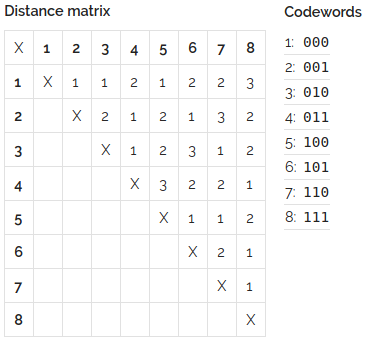
\includegraphics[scale=0.7]{../img/hamming1.png}
\caption{Hasil tabel jarak Hamming pada $(3,8,1)_2$}
\label{fig:hamming1}
\end{figure}

\begin{figure}
\centering
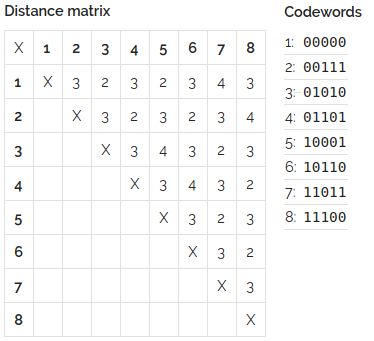
\includegraphics[scale=0.7]{../img/hamming2.png}
\caption{Hasil tabel jarak Hamming pada $(5,8,2)_2$}
\label{fig:hamming2}
\end{figure}